\definecolor{Pink}{RGB}{255,0,131}
\definecolor{Purple}{RGB}{166,115,255}
\definecolor{Yellow}{RGB}{224,237,0}
\definecolor{Green}{RGB}{0,100,0}

    % Pagina 16%
    \begin{frame}{Tipos de ambiente}
        \begin{figure}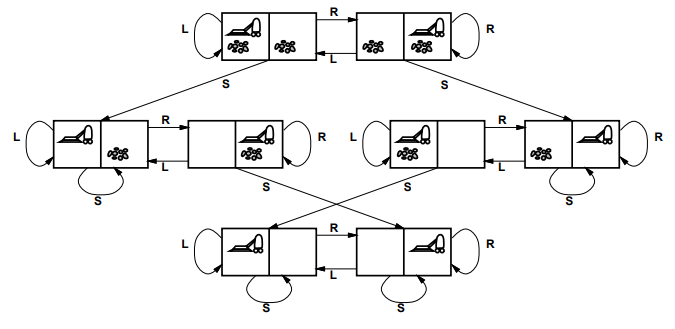
\includegraphics[ width=85mm ]{images/16_exampleVacuum.png}\end{figure}
        \small{
            \textcolor{Pink}{\underline{¿Estados?}}: Suciedad como entero y ubicacion del robot \\          \hspace{1.8cm} (ignore las \textcolor{Green}{cantidades} de suciedad, etc.) \\
            \textcolor{Pink}{\underline{¿Acciones?}}: \textcolor{Purple}{$Izquierda, Derecha, Aspirar, %
            Sin \hspace{0.1cm}acciones$} \\
            \textcolor{Pink}{\underline{¿Estado objetivo?}}: \\
            \textcolor{Pink}{\underline{¿Costo de ruta?}}: 
        }
        \break\break\break\break\break
    \end{frame}
